% Don't touch this %%%%%%%%%%%%%%%%%%%%%%%%%%%%%%%%%%%%%%%%%%%
\documentclass[12pt]{article}
\usepackage{fullpage}
\usepackage[left=1in,top=1in,right=1in,bottom=1in,headheight=3ex,headsep=3ex]{geometry}
\usepackage{graphicx}
\usepackage{float}
\usepackage{array}


\newcommand{\blankline}{\quad\pagebreak[2]}
%%%%%%%%%%%%%%%%%%%%%%%%%%%%%%%%%%%%%%%%%%%%%%%%%%%%%%%%%%%%%%

% Modify Course title, instructor name, semester here %%%%%%%%

\title{Review II}
\author{PHY250 - Fall 2021}
\date{}

%%%%%%%%%%%%%%%%%%%%%%%%%%%%%%%%%%%%%%%%%%%%%%%%%%%%%%%%%%%%%%

% Don't touch this %%%%%%%%%%%%%%%%%%%%%%%%%%%%%%%%%%%%%%%%%%%
\usepackage[sc]{mathpazo}
%\linespread{1.05} % Palatino needs more leading (space between lines)
\usepackage[T1]{fontenc}
\usepackage[mmddyyyy]{datetime}% http://ctan.org/pkg/datetime
\usepackage{advdate}% http://ctan.org/pkg/advdate
\newdateformat{syldate}{\twodigit{\THEMONTH}/\twodigit{\THEDAY}}
\newsavebox{\MONDAY}\savebox{\MONDAY}{Mon}% Mon
\newcommand{\week}[1]{%
%  \cleardate{mydate}% Clear date
% \newdate{mydate}{\the\day}{\the\month}{\the\year}% Store date
  \paragraph*{\kern-2ex\quad #1, \syldate{\today} - \AdvanceDate[4]\syldate{\today}:}% Set heading  \quad #1
%  \setbox1=\hbox{\shortdayofweekname{\getdateday{mydate}}{\getdatemonth{mydate}}{\getdateyear{mydate}}}%
  \ifdim\wd1=\wd\MONDAY
    \AdvanceDate[7]
  \else
    \AdvanceDate[7]
  \fi%
}
%\usepackage{setspace}
\usepackage{multicol}
%\usepackage{indentfirst}
\usepackage{fancyhdr,lastpage}
\usepackage{url}
\pagestyle{fancy}
\usepackage{hyperref}
\usepackage{lastpage}
\usepackage{amsmath}
\usepackage{layout}

\lhead{}
\chead{}
%%%%%%%%%%%%%%%%%%%%%%%%%%%%%%%%%%%%%%%%%%%%%%%%%%%%%%%%%%%%%%

% Modify header here %%%%%%%%%%%%%%%%%%%%%%%%%%%%%%%%%%%%%%%%%
%\rhead{\footnotesize Text in header}

%%%%%%%%%%%%%%%%%%%%%%%%%%%%%%%%%%%%%%%%%%%%%%%%%%%%%%%%%%%%%%
% Don't touch this %%%%%%%%%%%%%%%%%%%%%%%%%%%%%%%%%%%%%%%%%%%
\lfoot{}
\cfoot{\small \thepage/\pageref*{LastPage}}
\rfoot{}

\usepackage{array, xcolor}
\usepackage{color,hyperref}
\definecolor{clemsonorange}{HTML}{EA6A20}
\hypersetup{colorlinks,breaklinks,linkcolor=clemsonorange,urlcolor=clemsonorange,anchorcolor=clemsonorange,citecolor=black}

\begin{document}

\maketitle




% First Section %%%%%%%%%%%%%%%%%%%%%%%%%%%%%%%%%%%%%%%%%%%%


\newcounter{example}
\setcounter{example}{1}

\section*{Exercise \theexample}
Suppose the top surface of the vessel is
subjected to an external gauge pressure P2. (a) Derive a
formula for the speed, $v_1$ , at which the liquid flows from the
opening at the bottom into atmospheric pressure, $P_0$.
Assume the velocity of the liquid surface, $v_2$, is approximately
zero.

\vspace{5mm}

\begin{figure}[h!]
    \begin{center}
      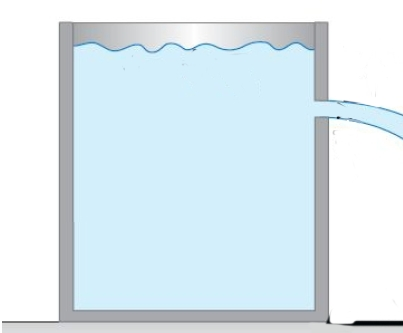
\includegraphics[height=2.5in]{images/1.jpg}
    \end{center}
  \end{figure}

% % First Section %%%%%%%%%%%%%%%%%%%%%%%%%%%%%%%%%%%%%%%%%%%%
% \stepcounter{example}

% \section*{Exercise \theexample}

% A scuba tank, when fully submerged, displaces 15.7 L of
% seawater. The tank itself has a mass of 14.0 kg and, when
% “full,” contains 3.00 kg of air. Assuming only a weight and
% buoyant force act, determine the net force (magnitude and
% direction) on the fully submerged tank at the beginning of a
% dive (when it is full of air) and at the end of a dive (when it
% no longer contains any air).

% First Section %%%%%%%%%%%%%%%%%%%%%%%%%%%%%%%%%%%%%%%%%%%%
\stepcounter{example}

\section*{Exercise \theexample}

Water stands at a height $h$ behind a vertical dam of
uniform width $b$. (a) Use integration to show that the total
force of the water on the dam is $F=\frac{1}{2}\rho g h^2 b$. (b) Show
that the torque about the base of the dam due to this force
can be considered to act with a lever arm equal to $h/3$.
(c) For a freestanding concrete dam of uniform thickness $t$ and
height $h$, what minimum thickness is needed to prevent
overturning? Do you need to add in atmospheric pressure
for this last part? Explain.


% First Section %%%%%%%%%%%%%%%%%%%%%%%%%%%%%%%%%%%%%%%%%%%%
\stepcounter{example}

\section*{Exercise \theexample}

A plywood disk of radius $20.0 cm$ and mass $2.20 kg$
has a small hole drilled through
it, $2.00 cm$ from its edge. The disk is hung
from the wall by means of a
metal pin through the hole, and
is used as a pendulum. What is
the period of this pendulum? ($I_{CM}=\frac{1}{2}MR^2$).


% First Section %%%%%%%%%%%%%%%%%%%%%%%%%%%%%%%%%%%%%%%%%%%%
\stepcounter{example}

\section*{Exercise \theexample}


One end of a horizontal string of linear density
$6.6 \times 10^{-4} kg/m$ is attached to a small-amplitude mechanical
$120-Hz$ oscillator. The string passes over a pulley, a
distance $\ell = 1.50 ~m$ away, and weights are hung from this
end. What mass $m$ must be hung from this end of
the string to produce (a) one loop, (b) two loops, and
(c) five loops of a standing wave? Assume the string at the
oscillator is a node, which is


\begin{figure}[h!]
  \begin{center}
    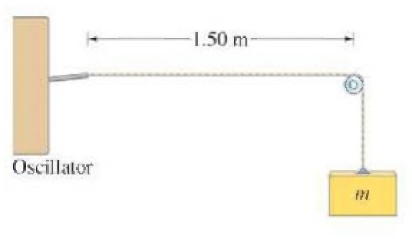
\includegraphics[height=2.5in]{images/2.jpg}
  \end{center}
\end{figure}

% First Section %%%%%%%%%%%%%%%%%%%%%%%%%%%%%%%%%%%%%%%%%%%%
\newcounter{questions}
\setcounter{questions}{1}

\stepcounter{example}

\section*{Question \thequestions}

A maintenance crew is working on a section of a three-lane highway, leaving only one
lane open to traffic. The result is much slower traffic flow (a traffic jam). Do cars on a
highway behave like
\vspace{5mm}
\\
(i) the molecules of an incompressible fluid or\\
(ii) the molecules of a compressible fluid?

% First Section %%%%%%%%%%%%%%%%%%%%%%%%%%%%%%%%%%%%%%%%%%%%
\stepcounter{questions}

\section*{Question \thequestions}

Mercury is less dense at high temperatures than at low temperatures. Suppose you move
a mercury barometer from the cold interior of a tightly sealed refrigerator to outdoors
on a hot summer day. You find that the column of mercury remains at the same height
in the tube. Compared to the air pressure inside the refrigerator, is the air pressure outdoors
\vspace{5mm}
\\
(i) higher,\\
(ii) lower, or\\
(iii) the same?

% First Section %%%%%%%%%%%%%%%%%%%%%%%%%%%%%%%%%%%%%%%%%%%%
\stepcounter{questions}

\section*{Question \thequestions}

Explain the difference between the speed of a transverse wave
traveling down a cord and the speed of a tiny piece of the cord.

% First Section %%%%%%%%%%%%%%%%%%%%%%%%%%%%%%%%%%%%%%%%%%%%
\stepcounter{questions}

\section*{Question \thequestions}

If we knew that energy was being transmitted from one place
to another, how might we determine whether the energy was
being carried by particles (material objects) or by waves?

% First Section %%%%%%%%%%%%%%%%%%%%%%%%%%%%%%%%%%%%%%%%%%%%
\stepcounter{questions}

\section*{Question \thequestions}

When a sinusoidal wave crosses the boundary between two
sections of cord, the frequency does not change
(although the wavelength and velocity do change). Explain why.


\end{document}


